%!TEX program = xelatex
\documentclass[cs4size,punct]{ctexart}
\usepackage{titling}
\usepackage[a4paper, left=30mm, right=20mm, top=35mm, bottom=25mm, headheight=20pt]{geometry}
\usepackage{fancyhdr, graphicx, xpatch, layout}
\usepackage{booktabs}
\usepackage{amsmath}
\usepackage{pdfpages}
\usepackage{float}
% \usepackage{cite}
\usepackage{enumitem}
\usepackage{titlesec}
\usepackage{tabularx}
\usepackage{chngcntr}
\usepackage{listings}
\usepackage{cleveref}
\usepackage[titles]{tocloft}
\usepackage[labelsep=space]{caption}
\usepackage[square, numbers, sort, comma]{natbib}
\usepackage{lmodern}
\usepackage{indentfirst}
\usepackage{xcolor} 
% 参考文献行间距
\setlength{\bibsep}{-1pt}

%设置字体
\setmainfont{Times New Roman} % set all eng font
\songti
\zihao{-4}
\CTEXsetup[format+={\mdseries\zihao{3}\heiti}]{section}
\CTEXsetup[format+={\mdseries\zihao{-4}\heiti}]{subsection}
\CTEXsetup[format+={\mdseries\zihao{-4}\heiti}]{subsubsection}

%设置间距
\linespread{1.6}
\titlespacing{\section}{0bp}{0.5em}{0.5em}
\titlespacing{\subsection}{0bp}{0.5em}{0.5em}
\titlespacing{\subsubsection}{0.5bp}{0.5em}{0.5em}


% 图表每章重新编号
\counterwithin{table}{section}
\counterwithin{figure}{section}

%列表样式
\setlist[enumerate,1]{label=\arabic*、, wide, labelsep=-0.3em, itemsep=-0.2ex, topsep=0pt, partopsep=0pt, parsep=0pt}
\setlist[enumerate,2]{label=(\arabic*)\ , wide, labelsep=0em, itemsep=0ex, topsep=0pt, partopsep=0pt, parsep=0pt}

\pagenumbering{Roman} %目录页码为罗马数字
%页眉
\pagestyle{fancy}
% \lhead{	\setlength{\unitlength}{1mm}
%         \begin{picture}(0,0)
%         \put(0,0){\includegraphics[height=1.7cm]{images/logo.pdf}}
%         \end{picture}
% }

\chead{\zihao{-4}\heiti  东北大学秦皇岛分校本科生毕业设计(论文)}
% \bfseries

\cfoot{\thepage}
\lhead{}
\rhead{}
\renewcommand{\headrulewidth}{0.4pt}
%%页眉

%% lstlisting 样式
\def\inline{\lstinline[basicstyle=\ttfamily,breaklines=true]}
\lstset{
	basicstyle=\ttfamily\zihao{5},
	xleftmargin=2em,
    breaklines=true,
    frame={tb},
    belowcaptionskip=1em
}

%自定义命令
\newcommand{\scite}[1]{\textsuperscript{\cite{#1}}} %cite样式

\DeclareCaptionFormat{myformat}{\zihao{5}\selectfont#1#2#3}
\captionsetup{format=myformat}

\begin{document}

%引用样式
\counterwithin{lstlisting}{section}
\renewcommand{\lstlistingname}{代码清单}
\crefname{listing}{代码清单}{代码清单}
\Crefname{listing}{代码清单}{代码清单}
\crefname{table}{表}{表}
\Crefname{table}{表}{表}
\crefname{figure}{图}{图}
\Crefname{figure}{图}{图}

\begin{titlepage}
	
\includepdf[fitpaper]{images/cover-1.pdf}
\end{titlepage}


\begin{titlepage}
	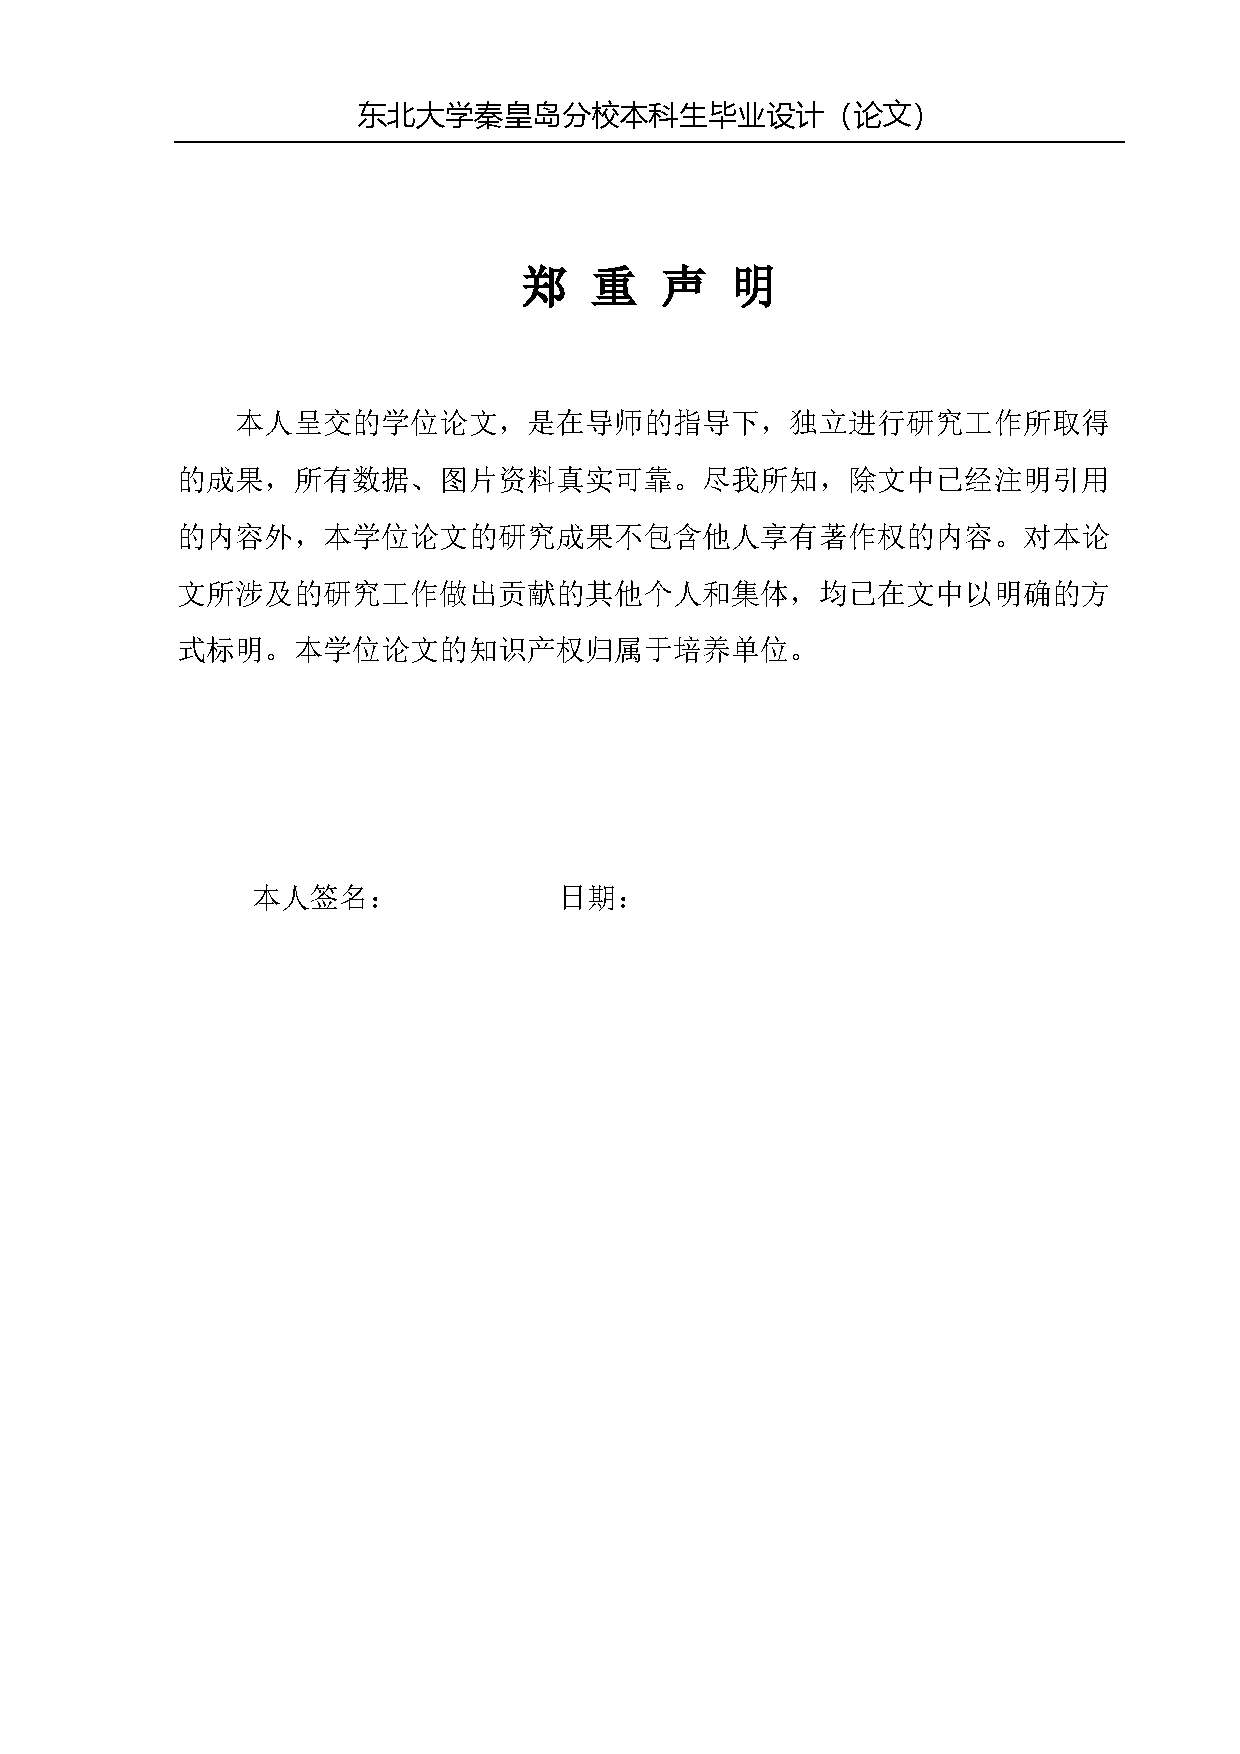
\includepdf[fitpaper]{images/cover-2.pdf}
\end{titlepage}

\section*{xxxx-xxxx即时通讯系统的设计与实现}
\section*{摘\ \ \ \ 要}

	这是一段摘要
	

\paragraph{关键词:} 关键词,关键词,关键词,关键词

\clearpage


\section*{Design and Implementation of xxxx-xxxx}

\hfill Author: xxxx

\hfill Tutor: xxxx

\section*{Abstract}

	这是一段英文摘要
	
\paragraph{Keywords: }xxxx,xxxx,xxxx,xxxx








%目录样式
% \renewcommand{\cftdot}{\ensuremath{\ast}}
\renewcommand{\cftsecleader}{\cftdotfill{\cftdotsep}}
\newcommand\mydot[1]{\scalebox{#1}{.}}
\renewcommand\cftdot{\mydot{0.8}}
\renewcommand\cftdotsep{1}
% \CTEXoptions[contentsname={\zihao{-4}目录}]
\tableofcontents

\pagenumbering{arabic} %正文页码为阿拉伯数字
\section{绪论}
  	\subsection{课题的背景和意义}
	
	即时通讯(Instant Messaging,简称 IM)这种通讯手段已经融入生活的各个方面,随着近年来各种移动 IM 应用的流行,即时通讯已经成为人与人之间交流的重要工具。尤其是近几年的快速发展,即时通讯的功能也日渐丰富,由最初的简单文字聊天逐渐扩展到图片、语音、视频等多种形式,成为集交流、资讯、娱乐、办公协作等一体的综合化信息平台。
	
	省略一段文字...
	
	
	\subsection{国内外即时通讯的发展状况}
	
	由于即时通讯软件的飞速发展和其特有的实时性、扩平台性、效率高等诸多优势,使之成为人们最喜爱的网络沟通手段之一。在移动互联网的范畴内,国内外涌现出大量的即时通讯软件,国内以腾讯的QQ、微信最受欢迎,国外最著名的当属 WhatsApp,即时通讯技术在手机端展现出强大的活力。
	
	省略一段文字...
	
  	\subsection{课题研究的主要方法及内容}

 	本课题主要工作是...

  	本课题主要包含以下几个方面内容:
  
  	\begin{enumerate}
  
    \item 调研主流即时通讯软件的功能...
    
    \item 深入研究...
    
    \item 设计实现...

    \item 实现整个...
    
  	\end{enumerate}

  	\subsection{论文组织结构}
  
  	本文主要围绕相关技术选型,需求分析,系统整体设计、详细设计,部署与测试等方面来进行论述,共分为6章,各章内容如下:
	
	第1章...
	
    第2章...
    
    第3章...
    
    第4章... 
       
    第5章...
    
    第6章...
    
    为了更好的理解 ...
    
\clearpage
\section{相关背景知识介绍}

	\subsection{开发工具和环境}
  
  	\begin{enumerate}[fullwidth,itemindent=2em,listparindent=2em]

  		\item 开发工具:Android Studio
 	
 		Android Studio 省略一段文字...
 			
		\item   开发环境:Android SDK
	
		SDK(Software Development Kit)省略一段文字...
  
  	
  	\end{enumerate}
     
    \subsection{环信即时通讯云}
    
    对于移动端来说,省略一段文字...
        
    环信成立于2013年4月,省略一段文字...   ,引用的用法...环信\scite{cite_环信}。
    
    \subsection{涉及的开源库}
	
	\begin{enumerate}[fullwidth,itemindent=2em,listparindent=2em]
	
		\item 网络请求库 Retrofit 2.0
		
		Retrofit 是一个 Square 开发的类型安全的 省略一段文字...
				
		\item 视图绑定库 ButterKnife
		
		ButterKnife 是一个基于注解的视图绑定库省略一段文字...
		
		\item 内存监控库 LeakCanary
		
		LeakCanary 是一个监测省略一段文字...	
		
		\item 日志工具库 Logger
		
		Logger 是一个简单省略一段文字...
		
		\item 二维码扫描库 ZXing
		
		ZXing 是一个省略一段文字...		
		
		\item 汉字转拼音库 TinyPinyin

		TinyPinyin 是一个省略一段文字省略一段文字省略一段文字省略一段文字省略一段文字省略一段文字省略一段文字省略一段文字省略一段文字省略一段文字省略一段文字省略一段文字省略一段文字省略一段文字省略一段文字省略一段文字省略一段文字省略一段文字省略一段文字省略一段文字省略一段文字省略一段文字省略一段文字省略一段文字		
			
	\end{enumerate}
	
	
\clearpage
\section{系统需求分析}
	\subsection{系统需求概述}
  
	作为一个即时通讯系统,省略一段文字省略一段文字省略一段文字省略一段文字省略一段文字省略一段文字省略一段文字省略一段文字省略一段文字省略一段文字省略一段文字省略一段文字省略一段文字省略一段文字省略一段文字省略一段文字省略一段文字省略一段文字省略一段文字省略一段文字省略一段文字省略一段文字省略一段文字省略一段文字... 性能需求\scite{cite_性能需求},整体需求如\Cref{demand analysis}所示。
	
     
	\begin{figure}[H]
		\centering
		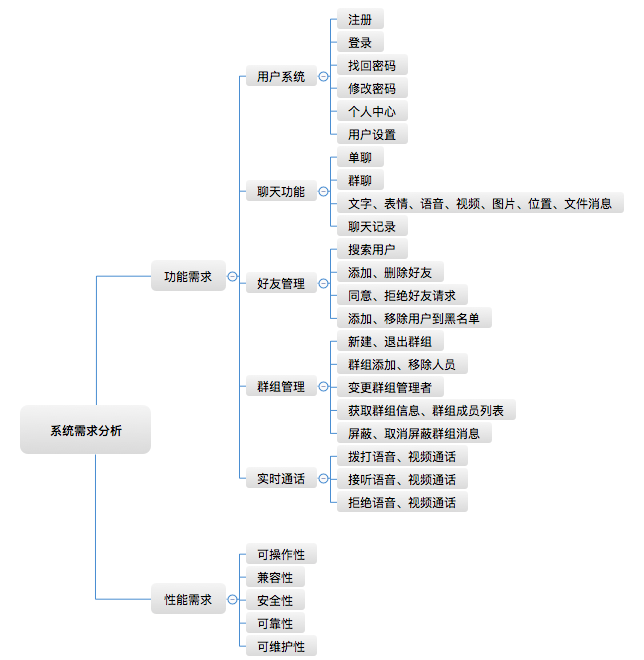
\includegraphics[width=0.95\textwidth]{images/demand_analysis}
		\caption{系统需求概述}
		\label{demand analysis}
	\end{figure}
     
     
	\subsection{功能需求分析}
  
	系统的功能性需求主要...,详细情况如下:
  
	\begin{enumerate}[fullwidth,itemindent=2em,listparindent=2em]
	
    \item 功能需求1

    	\begin{enumerate}
			\item 注册。省略一段文字省略一段文字省略一段文字省略一段文字省略一段文字省略一段文字省略一段文字省略一段文字省略一段文字省略一段文字省略一段文字省略一段文字省略一段文字省略一段文字省略一段文字省略一段文字省略一段文字省略一段文字省略一段文字省略一段文字省略一段文字省略一段文字省略一段文字省略一段文字
			\item 登录。省略一段文字省略一段文字省略一段文字省略一段文字省略一段文字省略一段文字省略一段文字省略一段文字省略一段文字省略一段文字省略一段文字省略一段文字省略一段文字省略一段文字省略一段文字省略一段文字省略一段文字省略一段文字省略一段文字省略一段文字省略一段文字省略一段文字省略一段文字省略一段文字
			\item 省略一段文字省略一段文字省略一段文字省略一段文字省略一段文字省略一段文字省略一段文字省略一段文字省略一段文字省略一段文字省略一段文字省略一段文字省略一段文字省
			
		\end{enumerate}

    \item 功能需求2
    
    	\begin{enumerate}
    
    		\item 省略一段文字省略一段文字省略一段文字省略一段文字省略一段文字省略一段文字省略一段文字省略一段文字省略一段文字省略一段文字省略一段文字省略一段文字省略一段文字省

    		\item 省略一段文字省略一段文字省略一段文字省略一段文字省略一段文字省略一段文字省略一段文字省略一段文字省略一段文字省略一段文字省略一段文字省略一段文字省略一段文字省
    		
    	\end{enumerate}
    

    \item 功能需求3
   
   		\begin{enumerate}
   			\item 省略一段文字省略一段文字省略一段文字省略一段文字省略一段文字省略一段文字省略一段文字省略一段文字省略一段文字省略一段文字省略一段文字省略一段文字省略一段文字省

    		\item 省略一段文字省略一段文字省略一段文字省略一段文字省略一段文字省略一段文字省略一段文字省略一段文字省略一段文字省略一段文字省略一段文字省略一段文字省略一段文字省
   		\end{enumerate}
   

    \item 功能需求4
    
    	\begin{enumerate}
    		\item 省略一段文字省略一段文字省略一段文字省略一段文字省略一段文字省略一段文字省略一段文字省略一段文字省略一段文字省略一段文字省略一段文字省略一段文字省略一段文字省

    		\item 省略一段文字省略一段文字省略一段文字省略一段文字省略一段文字省略一段文字省略一段文字省略一段文字省略一段文字省略一段文字省略一段文字省略一段文字省略一段文字省
    	\end{enumerate}
    	

    \item 功能需求5
    
    	\begin{enumerate}
    		\item 省略一段文字省略一段文字省略一段文字省略一段文字省略一段文字省略一段文字省略一段文字省略一段文字省略一段文字省略一段文字省略一段文字省略一段文字省略一段文字省

    		\item 省略一段文字省略一段文字省略一段文字省略一段文字省略一段文字省略一段文字省略一段文字省略一段文字省略一段文字省略一段文字省略一段文字省略一段文字省略一段文字省
    	\end{enumerate}

	\end{enumerate}
    
    
	\subsection{性能需求分析}

	\begin{enumerate}[fullwidth,itemindent=2em,listparindent=2em]
  
  	\item 性能需求1
  	
  	省略一段文字省略一段文字省略一段文字省略一段文字省略一段文字省略一段文字省略一段文字省略一段文字省略一段文字省略一段文字省略一段文字省略一段文字省略一段文字省  	
  	\item 性能需求2
  	
  	省略一段文字省略一段文字省略一段文字省略一段文字省略一段文字省略一段文字省略一段文字省略一段文字省略一段文字省略一段文字省略一段文字省略一段文字省略一段文字省
  	
  	\item 性能需求3
  	
  	省略一段文字省略一段文字省略一段文字省略一段文字省略一段文字省略一段文字省略一段文字省略一段文字省略一段文字省略一段文字省略一段文字省略一段文字省略一段文字省
  	
  	\item 性能需求4
  	
  	省略一段文字省略一段文字省略一段文字省略一段文字省略一段文字省略一段文字省略一段文字省略一段文字省略一段文字省略一段文字省略一段文字省略一段文字省略一段文字省  	
  	\item 性能需求5
  	
  	省略一段文字省略一段文字省略一段文字省略一段文字省略一段文字省略一段文字省略一段文字省略一段文字省略一段文字省略一段文字省略一段文字省略一段文字省略一段文字省
  
  
	\end{enumerate}


\clearpage
\section{系统总体设计}

	系统总体结构组成如\Cref{overall_structure}所示,省略一段文字省略一段文字省略一段文字省略一段文字省略一段文字省略一段文字省略一段文字省略一段文字省略一段文字省略一段文字省略一段文字省略一段文字省略一段文字省
		
	\begin{figure}[H]
		\centering
		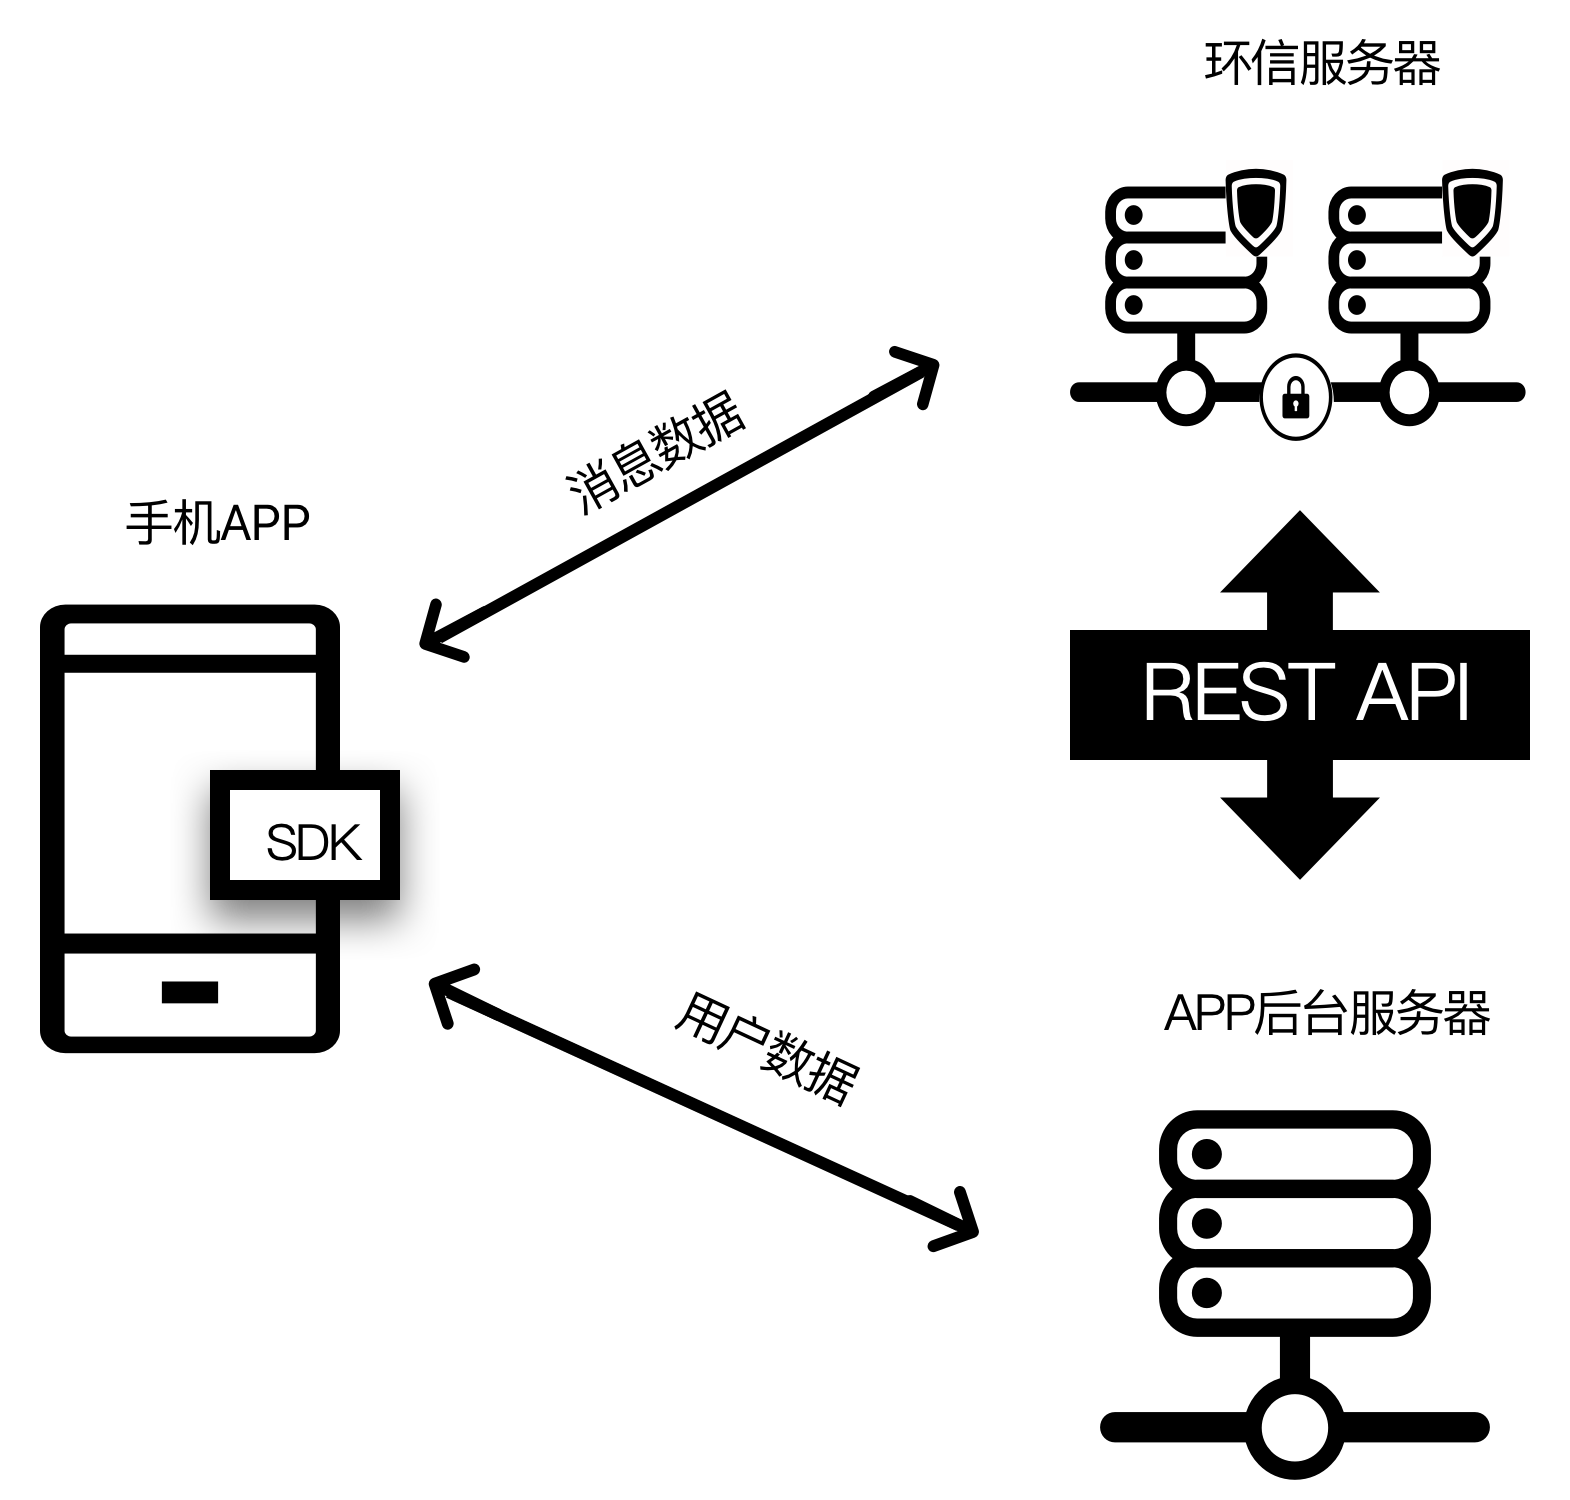
\includegraphics[width=0.80\textwidth]{images/all_design}
		\caption{系统总体结构组成}
		\label{overall_structure}
	\end{figure}
	
	\subsection{服务端总体设计}
	
		服务端的实现省略一段文字省略一段文字省略一段文字省略一段文字省略一段文字省略一段文字省略一段文字省略一段文字省略一段文字省略一段文字省略一段文字省略一段文字省略一段文字省		  
		  
		 省略一段文字省略一段文字省略一段文字省略一段文字省略一段文字省略一段文字省略一段文字省略一段文字省略一段文字省略一段文字省略一段文字省略一段文字省略一段文字省
		 
		  		  
		  
	\subsection{客户端总体设计}
		
		客户端采用分层的架构进行设计,上层实现依赖于下层设计\scite{cite_分层设计},自下而上分为基础层、数据层、组件层、表现层、应用层,整体设计结构如\Cref{mobile_overall_design}所示。
	
	\begin{figure}[H]
		\centering
		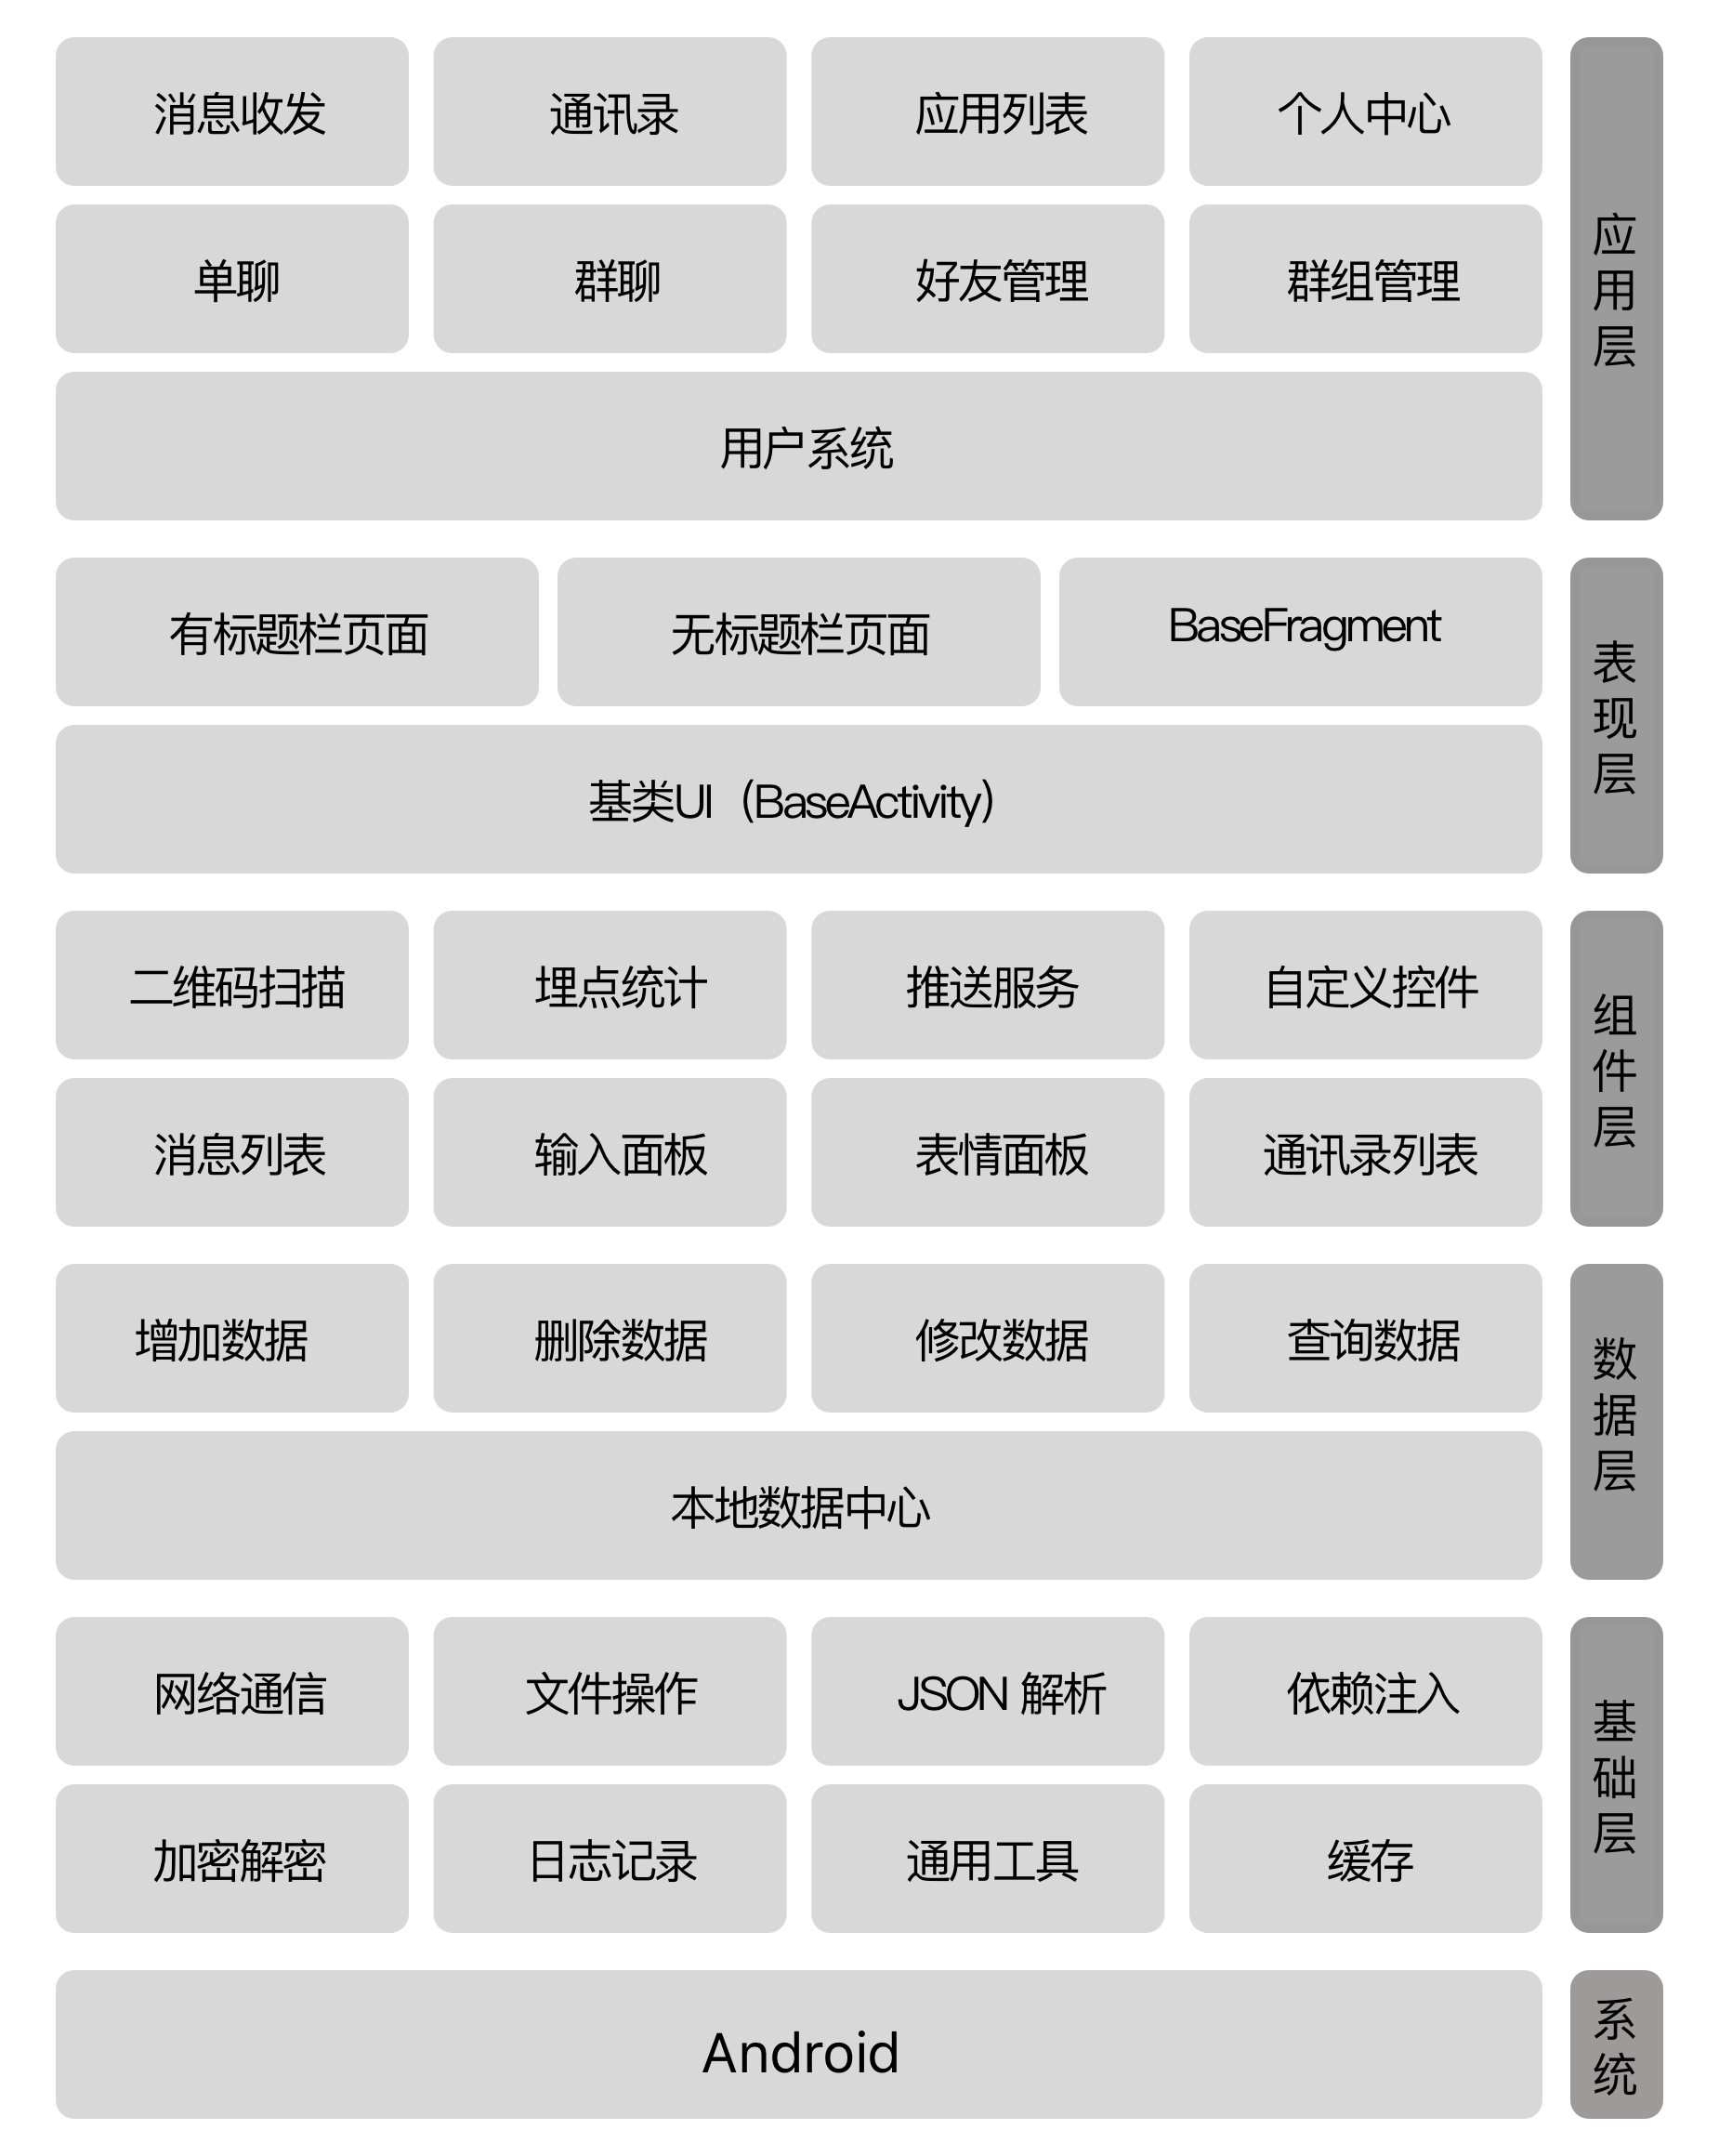
\includegraphics[width=0.95\textwidth]{images/mobile_design}
		\caption{移动端总体设计结构}
		\label{mobile_overall_design}
	\end{figure}


	\begin{enumerate}[fullwidth,itemindent=2em,listparindent=2em]
	
		\item 设计概述
		
		省略一段文字省略一段文字省略一段文字省略一段文字省略一段文字省略一段文字省略一段文字省略一段文字省略一段文字省略一段文字省略一段文字省略一段文字省略一段文字省
		
		省略一段文字省略一段文字省略一段文字省略一段文字省略一段文字省略一段文字省略一段文字省略一段文字省略一段文字省略一段文字省略一段文字省略一段文字省略一段文字省
		
		\item 设计概述
		
		省略一段文字省略一段文字省略一段文字省略一段文字省略一段文字省略一段文字省略一段文字省略一段文字省略一段文字省略一段文字省略一段文字省略一段文字省略一段文字省
		
		省略一段文字省略一段文字省略一段文字省略一段文字省略一段文字省略一段文字省略一段文字省略一段文字省略一段文字省略一段文字省略一段文字省略一段文字省略一段文字省

		\item 设计概述
		
		省略一段文字省略一段文字省略一段文字省略一段文字省略一段文字省略一段文字省略一段文字省略一段文字省略一段文字省略一段文字省略一段文字省略一段文字省略一段文字省
		
		省略一段文字省略一段文字省略一段文字省略一段文字省略一段文字省略一段文字省略一段文字省略一段文字省略一段文字省略一段文字省略一段文字省略一段文字省略一段文字省

			
		

	\end{enumerate}

	\subsection{数据库总体设计}

		
		省略一段文字省略一段文字省略一段文字省略一段文字省略一段文字省略一段文字省略一段文字省略一段文字省略一段文字省略一段文字省略一段文字省,表格使用,表格使用,表格使用,表格使用,表格使用,表格使用,如\Cref{tab:db_table_user}所示。
	
		\begin{table}[H]
		\centering
		\caption{User 用户表}
		\zihao{5}
		\label{tab:db_table_user}
		\begin{tabular}{p{0.21\textwidth}p{0.21\textwidth}p{0.21\textwidth}p{0.21\textwidth}}
		\hline
		字段          & 数据类型         & 字段含义   & 约束条件     \\ \hline
		id          & INT(11)      & 用户ID & 主键、非空、自增 \\
		im\_id      & VARCHAR(256) & 环信ID & 唯一       \\ 
		account     & VARCHAR(45)  & 用户名  & 唯一       \\ 
		nick\_name  & VARCHAR(100) & 昵称   & 无        \\
		password    & VARCHAR(256) & 密码   & 非空       \\ 
		email       & VARCHAR(45)  & 邮箱   & 无        \\
		mobile      & VARCHAR(45)  & 手机号  & 唯一        \\ 
		sex         & INT(11)      & 性别   & 无        \\ 
		signature   & VARCHAR(512) & 签名   & 无        \\
		avatar      & VARCHAR(256) & 头像   & 无        \\
		is\_deleted & TINYINT(4)   & 删除标志 & 无        \\ \hline
		\end{tabular}
		\end{table}
		
 \clearpage
\section{系统详细设计}

	系统详细设计实现省略一段文字省略一段文字省略一段文字省略一段文字省略一段文字省略一段文字省略一段文字省略一段文字省略一段文字省略一段文字省略一段文字省略一段文字省略一段文字省省略一段文字省略一段文字省略一段文字省略一段文字省略一段文字省略一段文字省略一段文字省略一段文字省略一段文字省略一段文字省略一段文字省略一段文字省略一段文字省

  \subsection{基础层详细设计}
	
   	\subsubsection{网络通信的实现}

		实现省略一段文字省略一段文字省略一段文字省略一段文字省略一段文字省略一段文字省略一段文字省略一段文字省略一段文字省略一段文字省略一段文字省略一段文字省略一段文字省省略一段文字省略一段文字省略一段文字省略一段文字省略一段文字省略一段文字省略一段文字省略一段文字省略一段文字省略一段文字省略一段文字省略一段文字省略一段文字省

		
		这里以\Cref{code_api_service} 为例,代码块使用示例
		
		
		\begin{lstlisting}[caption=APIService , label=code_api_service]
 /** 
  * 登录 
  */
 @POST("user/login")
 Call<APIResponse<LoginResponse>> login(@Body LoginRequest request);

 /** 
  * 获取单个用户详细信息
  */
 @GET("user/{imid}/info")
 Call<APIResponse<UserInfo>> getUserInfo(@Path("imid") String imId);
 
		\end{lstlisting}                 

	
			
   	\subsubsection{日志记录的实现}
    
    实现省略一段文字省略一段文字省略一段文字省略一段文字省略一段文字省略一段文字省略一段文字省略一段文字省略一段文字省略一段文字省略一段文字省略一段文字省略一段文字省省略一段文字省略一段文字省略一段文字省略一段文字省略一段文字省略一段文字省略一段文字省略一段文字省略一段文字省略一段文字省略一段文字省略一段文字省略一段文字省日志记录输出样式如\Cref{img_log_sample}所示。
    
    \begin{figure}[H]
    	\centering
    	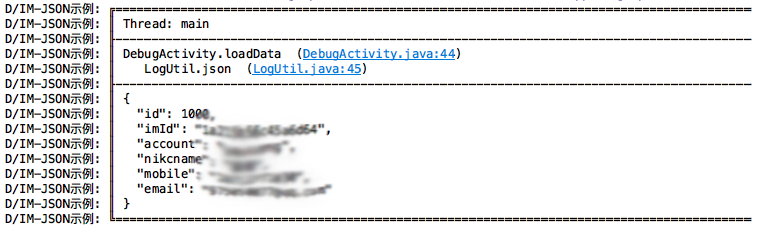
\includegraphics[width=0.95\textwidth]{images/log_sample}
    	\caption{日志信息示例}
    	\label{img_log_sample}
    \end{figure}
    
    
   	\subsubsection{加密解密的实现}
    
    实现省略一段文字省略一段文字省略一段文字省略一段文字省略一段文字省略一段文字省略一段文字省略一段文字省略一段文字省略一段文字省略一段文字省略一段文字省略一段文字省省略一段文字省略一段文字省略一段文字省略一段文字省略一段文字省略一段文字省略一段文字省略一段文字省略一段文字省略一段文字省略一段文字省略一段文字省略一段文字省
        
   	\subsubsection{缓存的实现}
   	
   	实现省略一段文字省略一段文字省略一段文字省略一段文字省略一段文字省略一段文字省略一段文字省略一段文字省略一段文字省略一段文字省略一段文字省略一段文字省略一段文字省省略一段文字省略一段文字省略一段文字省略一段文字省略一段文字省略一段文字省略一段文字省略一段文字省略一段文字省略一段文字省略一段文字省略一段文字省略一段文字省
   	   	
   	\subsubsection{文件操作工具的实现}
   	
   	文件操作模块定义了全局工具类 FileUtil,内部实现了常用的文件操作方法以及格式化输出文件大小的方法。常用文件操作方法包含判断文件是否存在、读文件、写文件、移动文件、复制文件、删除文件、创建文件、文件重命名、获取文件名称、判断是否有文件夹、调用系统方式打开文件、将字符串以不同形式的编码写入文件中。格式化文件大小主要是将文件的大小转换为更直观的形式,如:15KB、0.38M、1.52G。
   	
   	\subsubsection{JSON解析的实现}

	实现省略一段文字省略一段文字省略一段文字省略一段文字省略一段文字省略一段文字省略一段文字省略一段文字省略一段文字省略一段文字省略一段文字省略一段文字省略一段文字省省略一段文字省略一段文字省略一段文字省略一段文字省略一段文字省略一段文字省略一段文字省略一段文字省略一段文字省略一段文字省略一段文字省略一段文字省略一段文字省
	
  \subsection{数据层详细设计}

	实现省略一段文字省略一段文字省略一段文字省略一段文字省略一段文字省略一段文字省略一段文字省略一段文字省略一段文字省略一段文字省略一段文字省略一段文字省略一段文字省省略一段文字省略一段文字省略一段文字省略一段文字省略一段文字省略一段文字省略一段文字省略一段文字省略一段文字省略一段文字省略一段文字省略一段文字省略一段文字省
		 
	
	实现省略一段文字省略一段文字省略一段文字省略一段文字省略一段文字省略一段文字省略一段文字省略一段文字省略一段文字省略一段文字省略一段文字省略一段文字省略一段文字省省略一段文字省略一段文字省略一段文字省略一段文字省略一段文字省略一段文字省略一段文字省略一段文字省略一段文字省略一段文字省略一段文字省略一段文字省略一段文字省
	
	
  \subsection{组件层详细设计}

   	\subsubsection{二维码扫描的实现}
   	
	实现省略一段文字省略一段文字省略一段文字省略一段文字省略一段文字省略一段文字省略一段文字省略一段文字省略一段文字省略一段文字省略一段文字省略一段文字省略一段文字省省略一段文字省略一段文字省略一段文字省略一段文字省略一段文字省略一段文字省略一段文字省略一段文字省略一段文字省略一段文字省略一段文字省略一段文字省略一段文字省

   	\subsubsection{消息列表的实现}
	
	实现省略一段文字省略一段文字省略一段文字省略一段文字省略一段文字省略一段文字省略一段文字省略一段文字省略一段文字省略一段文字省略一段文字省略一段文字省略一段文字省省略一段文字省略一段文字省略一段文字省略一段文字省略一段文字省略一段文字省略一段文字省略一段文字省略一段文字省略一段文字省略一段文字省略一段文字省略一段文字省
	
   	\subsubsection{输入面板的实现}
   	
   	实现省略一段文字省略一段文字省略一段文字省略一段文字省略一段文字省略一段文字省略一段文字省略一段文字省略一段文字省略一段文字省略一段文字省略一段文字省略一段文字省省略一段文字省略一段文字省略一段文字省略一段文字省略一段文字省略一段文字省略一段文字省略一段文字省略一段文字省略一段文字省略一段文字省略一段文字省略一段文字省,输入面板具体样式如\Cref{input_panel}所示。
   	
   	\begin{figure}[H]
		\centering
		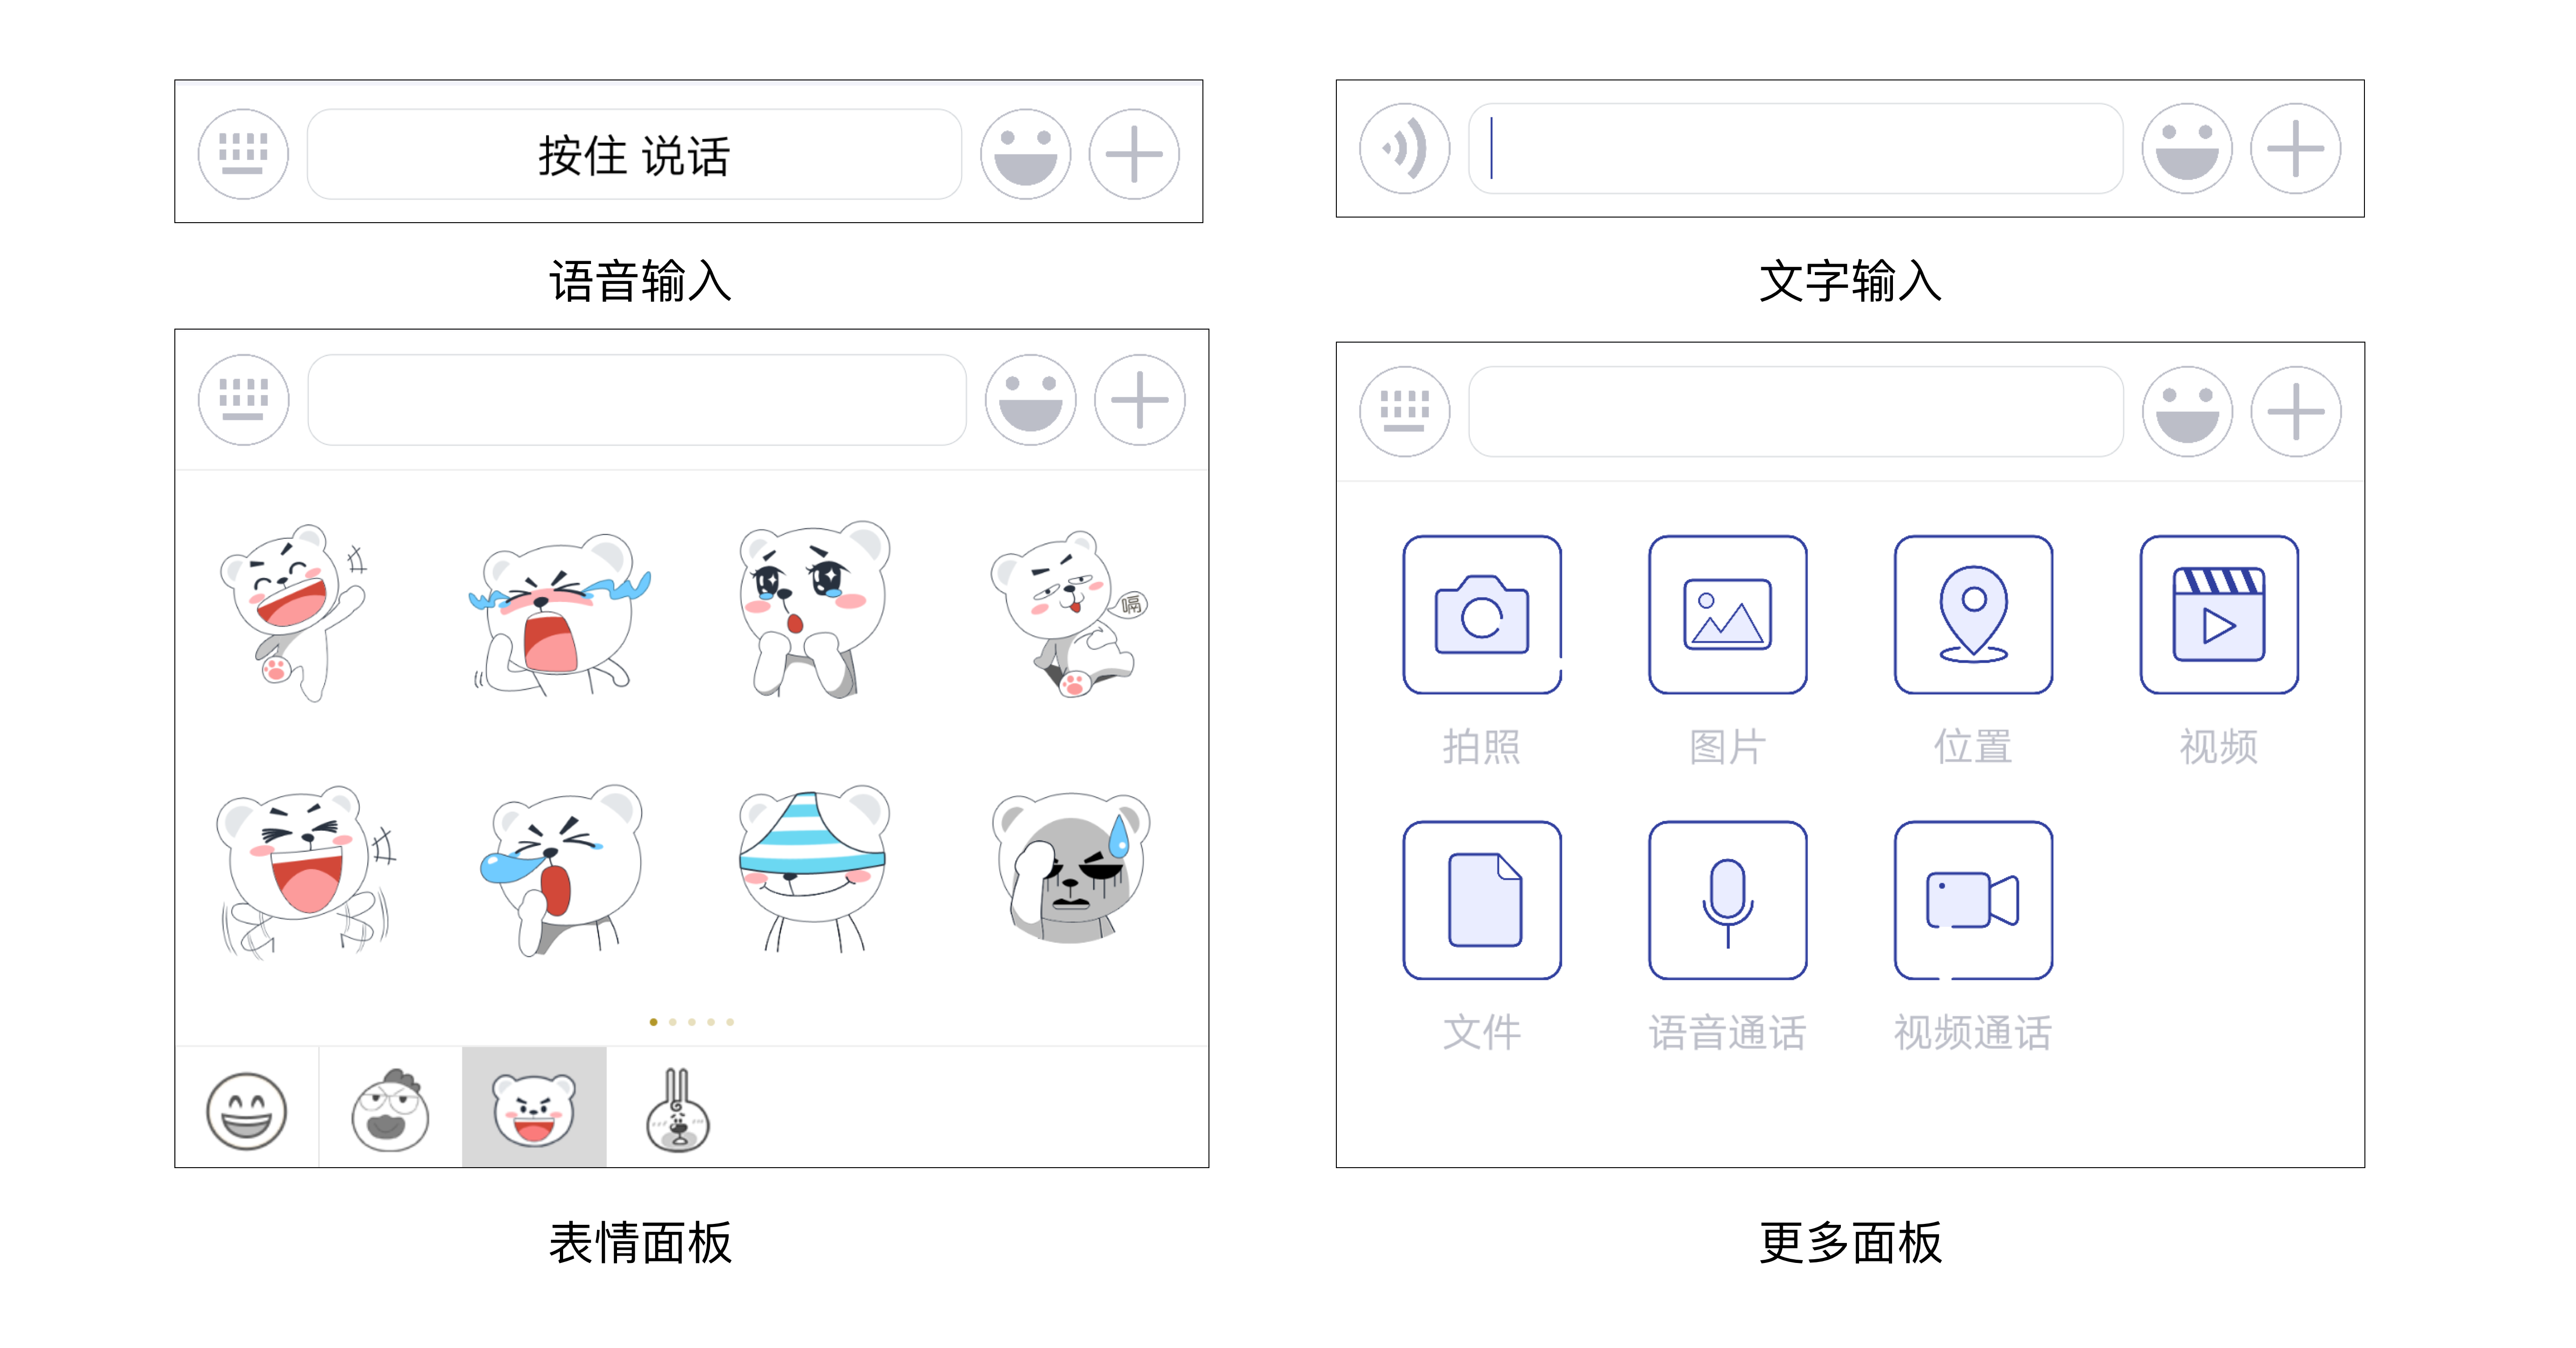
\includegraphics[width=0.95\textwidth]{images/input_panel}
		\caption{输入面板样式}
		\label{input_panel}
	\end{figure}
	
	
   	\subsubsection{表情面板的实现}
   	
   	实现省略一段文字省略一段文字省略一段文字省略一段文字省略一段文字省略一段文字省略一段文字省略一段文字省略一段文字省略一段文字省略一段文字省略一段文字省略一段文字省省略一段文字省略一段文字省略一段文字省略一段文字省略一段文字省略一段文字省略一段文字省略一段文字省略一段文字省略一段文字省略一段文字省略一段文字省略一段文字省   	
   	   	   	
   	\subsubsection{更多面板的实现}
   	
   	实现省略一段文字省略一段文字省略一段文字省略一段文字省略一段文字省略一段文字省略一段文字省略一段文字省略一段文字省略一段文字省略一段文字省略一段文字省略一段文字省省略一段文字省略一段文字省略一段文字省略一段文字省略一段文字省略一段文字省略一段文字省略一段文字省略一段文字省略一段文字省略一段文字省略一段文字省略一段文字省
   	    
   	\subsubsection{通讯录列表的实现}
   	
   	实现省略一段文字省略一段文字省略一段文字省略一段文字省略一段文字省略一段文字省略一段文字省略一段文字省略一段文字省略一段文字省略一段文字省略一段文字省略一段文字省省略一段文字省略一段文字省略一段文字省略一段文字省略一段文字省略一段文字省略一段文字省略一段文字省略一段文字省略一段文字省略一段文字省略一段文字省略一段文字省
    
	\subsubsection{埋点统计的实现}
	
	实现省略一段文字省略一段文字省略一段文字省略一段文字省略一段文字省略一段文字省略一段文字省略一段文字省略一段文字省略一段文字省略一段文字省略一段文字省略一段文字省省略一段文字省略一段文字省略一段文字省略一段文字省略一段文字省略一段文字省略一段文字省略一段文字省略一段文字省略一段文字省略一段文字省略一段文字省略一段文字省
		
          

  \subsection{表现层详细设计}
	
	  \subsubsection{Activity 基类的实现}
	  
		实现省略一段文字省略一段文字省略一段文字省略一段文字省略一段文字省略一段文字省略一段文字省略一段文字省略一段文字省略一段文字省略一段文字省略一段文字省略一段文字省省略一段文字省略一段文字省略一段文字省略一段文字省略一段文字省略一段文字省略一段文字省略一段文字省略一段文字省略一段文字省略一段文字省略一段文字省略一段文字省
	  		

	  
	  	  
	  \subsubsection{Fragment 基类的实现}
	  
		实现省略一段文字省略一段文字省略一段文字省略一段文字省略一段文字省略一段文字省略一段文字省略一段文字省略一段文字省略一段文字省略一段文字省略一段文字省略一段文字省省略一段文字省略一段文字省略一段文字省略一段文字省略一段文字省略一段文字省略一段文字省略一段文字省略一段文字省略一段文字省略一段文字省略一段文字省略一段文字省
		

  \subsection{应用层详细设计}
  	
		\subsubsection{用户系统的实现}
		
		实现省略一段文字省略一段文字省略一段文字省略一段文字省略一段文字省略一段文字省略一段文字省略一段文字省略一段文字省略一段文字省略一段文字省略一段文字省略一段文字省省略一段文字省略一段文字省略一段文字省略一段文字省略一段文字省略一段文字省略一段文字省略一段文字省略一段文字省略一段文字省略一段文字省略一段文字省略一段文字省
		
		\subsubsection{聊天功能的实现}
		
		实现省略一段文字省略一段文字省略一段文字省略一段文字省略一段文字省略一段文字省略一段文字省略一段文字省略一段文字省略一段文字省略一段文字省略一段文字省略一段文字省省略一段文字省略一段文字省略一段文字省略一段文字省略一段文字省略一段文字省略一段文字省略一段文字省略一段文字省略一段文字省略一段文字省略一段文字省略一段文字省
				
	 	\subsubsection{好友管理的实现}
	 	
	 	实现省略一段文字省略一段文字省略一段文字省略一段文字省略一段文字省略一段文字省略一段文字省略一段文字省略一段文字省略一段文字省略一段文字省略一段文字省略一段文字省省略一段文字省略一段文字省略一段文字省略一段文字省略一段文字省略一段文字省略一段文字省略一段文字省略一段文字省略一段文字省略一段文字省略一段文字省略一段文字省
	 	
		\subsubsection{群组管理的实现}
		
		实现省略一段文字省略一段文字省略一段文字省略一段文字省略一段文字省略一段文字省略一段文字省略一段文字省略一段文字省略一段文字省略一段文字省略一段文字省略一段文字省省略一段文字省略一段文字省略一段文字省略一段文字省略一段文字省略一段文字省略一段文字省略一段文字省略一段文字省略一段文字省略一段文字省略一段文字省略一段文字省
		
		\subsubsection{通讯录的实现}
		
		实现省略一段文字省略一段文字省略一段文字省略一段文字省略一段文字省略一段文字省略一段文字省略一段文字省略一段文字省略一段文字省略一段文字省略一段文字省略一段文字省省略一段文字省略一段文字省略一段文字省略一段文字省略一段文字省略一段文字省略一段文字省略一段文字省略一段文字省略一段文字省略一段文字省略一段文字省略一段文字省
		
		\subsubsection{应用列表的实现}
		
		实现省略一段文字省略一段文字省略一段文字省略一段文字省略一段文字省略一段文字省略一段文字省略一段文字省略一段文字省略一段文字省略一段文字省略一段文字省略一段文字省省略一段文字省略一段文字省略一段文字省略一段文字省略一段文字省略一段文字省略一段文字省略一段文字省略一段文字省略一段文字省略一段文字省略一段文字省略一段文字省GridView更新。
		
		\subsubsection{个人中心的实现}
		
		实现省略一段文字省略一段文字省略一段文字省略一段文字省略一段文字省略一段文字省略一段文字省略一段文字省略一段文字省略一段文字省略一段文字省略一段文字省略一段文字省省略一段文字省略一段文字省略一段文字省略一段文字省略一段文字省略一段文字省略一段文字省略一段文字省略一段文字省略一段文字省略一段文字省略一段文字省略一段文字省

 \clearpage
\section{系统部署与测试}
	\subsection{服务端部署}
 
	实现省略一段文字省略一段文字省略一段文字省略一段文字省略一段文字省略一段文字省略一段文字省略一段文字省略一段文字省略一段文字省略一段文字省略一段文字省略一段文字省省略一段文字省略一段文字省略一段文字省略一段文字省略一段文字省略一段文字省略一段文字省略一段文字省略一段文字省略一段文字省略一段文字省略一段文字省略一段文字省
	
	 
	\subsection{客户端测试}
	
	\subsubsection{单元测试}
	
	实现省略一段文字省略一段文字省略一段文字省略一段文字省略一段文字省略一段文字省略一段文字省略一段文字省略一段文字省略一段文字省略一段文字省略一段文字省略一段文字省省略一段文字省略一段文字省略一段文字省略一段文字省略一段文字省略一段文字省略一段文字省略一段文字省略一段文字省略一段文字省略一段文字省略一段文字省略一段文字省

 	\subsubsection{功能测试}
 	
 	实现省略一段文字省略一段文字省略一段文字省略一段文字省略一段文字省略一段文字省略一段文字省略一段文字省略一段文字省略一段文字省略一段文字省略一段文字省略一段文字省省略一段文字省略一段文字省略一段文字省略一段文字省略一段文字省略一段文字省略一段文字省略一段文字省略一段文字省略一段文字省略一段文字省略一段文字省略一段文字省 	
 	
 	\subsubsection{深度兼容测试}
	
	实现省略一段文字省略一段文字省略一段文字省略一段文字省略一段文字省略一段文字省略一段文字省略一段文字省略一段文字省略一段文字省略一段文字省略一段文字省略一段文字省省略一段文字省略一段文字省略一段文字省略一段文字省略一段文字省略一段文字省略一段文字省略一段文字省略一段文字省略一段文字省略一段文字省略一段文字省略一段文字省


\clearpage
\section*{结论}
\addcontentsline{toc}{section}{结论}


	实现省略一段文字省略一段文字省略一段文字省略一段文字省略一段文字省略一段文字省略一段文字省略一段文字省略一段文字省略一段文字省略一段文字省略一段文字省略一段文字省省略一段文字省略一段文字省略一段文字省略一段文字省略一段文字省略一段文字省略一段文字省略一段文字省略一段文字省略一段文字省略一段文字省略一段文字省略一段文字省。总体上,完成了以下工作:
	
	\begin{enumerate}
	
		\item 调研了...
		
		\item 调研...
		
		\item 设计...
				
		\item 依据...	
		
		\item 对整个系统...

		 
	\end{enumerate}
	
	
	实现省略一段文字省略一段文字省略一段文字省略一段文字省略一段文字省略一段文字省略一段文字省略一段文字省略一段文字省略一段文字省略一段文字省略一段文字省略一段文字省省略一段文字省略一段文字省略一段文字省略一段文字省略一段文字省略一段文字省略一段文字省略一段文字省略一段文字省略一段文字省略一段文字省略一段文字省略一段文字省
\section*{致\ \ \ \ 谢}
\addcontentsline{toc}{section}{致\ \ \ \ 谢}

	实现省略一段文字省略一段文字省略一段文字省略一段文字省略一段文字省略一段文字省略一段文字省略一段文字省略一段文字省略一段文字省略一段文字省略一段文字省略一段文字省省略一段文字省略一段文字省略一段文字省略一段文字省略一段文字省略一段文字省略一段文字省略一段文字省略一段文字省略一段文字省略一段文字省略一段文字省略一段文字省

% \bibliographystyle{IEEEtran}
\bibliographystyle{gbt7714-2005}
% \bibliographystyle{thu}
% \bibliographystyle{cqu}
\nocite{*}
\addcontentsline{toc}{section}{参考文献}
\bibliography{citation}
% \setlength{\bibsep}{0pt plus 0.5em}

\appendix
% \renewcommand{\appendixname}{附录~\Alph{section}}
% \renewcommand{\appendixtocname}{附录}
% \addappheadtotoc
% \renewcommand{\appendixpagename}{\centering 附录}
% \appendixpage

% \begin{appendices}

% \heiti
% \zihao{3}

\section*{附\ \ \ \ 录\ \ \ }

\addcontentsline{toc}{section}{附\ \ \ \ 录}

\renewcommand{\thesubsection}{附录\Alph{subsection}}
% \renewcommand\thetable{\thesection.\arabic{table}}
% \renewcommand\thefigure{\arabic{figure}}

\newcommand{\appendsection}[1]{\titleformat*{\subsection}{\centering}\zihao{-4}\heiti\subsection{} {\centering\paragraph{#1}\mbox{}\\}\songti}
\newcommand{\appendchn}[1]{\titleformat*{\subsection}{\centering}\zihao{-4}\heiti\subsection*{中文译文\Alph{subsection}} {\centering\paragraph{#1}\mbox{}\\}\songti}

% \renewcommand{\figurename}{图 A.}
% \setcounter{figure}{0}

% \titlespacing*{\subsection}{-20pt}{*1.5}{*1.1}


\appendsection{Android, the world's most popular mobile platform}

	实现省略一段文字省略一段文字省略一段文字省略一段文字省略一段文字省略一段文字省略一段文字省略一段文字省略一段文字省略一段文字省略一段文字省略一段文字省略一段文字省省略一段文字省略一段文字省略一段文字省略一段文字省略一段文字省略一段文字省略一段文字省略一段文字省略一段文字省略一段文字省略一段文字省略一段文字省略一段文字省



\appendchn{Android,世界上最受欢迎的移动平台}

	实现省略一段文字省略一段文字省略一段文字省略一段文字省略一段文字省略一段文字省略一段文字省略一段文字省略一段文字省略一段文字省略一段文字省略一段文字省略一段文字省省略一段文字省略一段文字省略一段文字省略一段文字省略一段文字省略一段文字省略一段文字省略一段文字省略一段文字省略一段文字省略一段文字省略一段文字省略一段文字省


\appendsection{Android Application Fundamentals}

	实现省略一段文字省略一段文字省略一段文字省略一段文字省略一段文字省略一段文字省略一段文字省略一段文字省略一段文字省略一段文字省略一段文字省略一段文字省略一段文字省省略一段文字省略一段文字省略一段文字省略一段文字省略一段文字省略一段文字省略一段文字省略一段文字省略一段文字省略一段文字省略一段文字省略一段文字省略一段文字省

\subsubsection*{Application Components}

	实现省略一段文字省略一段文字省略一段文字省略一段文字省略一段文字省略一段文字省略一段文字省略一段文字省略一段文字省略一段文字省略一段文字省略一段文字省略一段文字省省略一段文字省略一段文字省略一段文字省略一段文字省略一段文字省略一段文字省略一段文字省略一段文字省略一段文字省略一段文字省略一段文字省略一段文字省略一段文字省components:

\subsubsection*{Activities}

	实现省略一段文字省略一段文字省略一段文字省略一段文字省略一段文字省略一段文字省略一段文字省略一段文字省略一段文字省略一段文字省略一段文字省略一段文字省略一段文字省省略一段文字省略一段文字省略一段文字省略一段文字省略一段文字省略一段文字省略一段文字省略一段文字省略一段文字省略一段文字省略一段文字省略一段文字省略一段文字省	
		
\subsubsection*{Services}

	实现省略一段文字省略一段文字省略一段文字省略一段文字省略一段文字省略一段文字省略一段文字省略一段文字省略一段文字省略一段文字省略一段文字省略一段文字省略一段文字省省略一段文字省略一段文字省略一段文字省略一段文字省略一段文字省略一段文字省略一段文字省略一段文字省略一段文字省略一段文字省略一段文字省略一段文字省略一段文字省

\subsubsection*{Broadcast receivers}

	实现省略一段文字省略一段文字省略一段文字省略一段文字省略一段文字省略一段文字省略一段文字省略一段文字省略一段文字省略一段文字省略一段文字省略一段文字省略一段文字省省略一段文字省略一段文字省略一段文字省略一段文字省略一段文字省略一段文字省略一段文字省略一段文字省略一段文字省略一段文字省略一段文字省略一段文字省略一段文字省
		
\subsubsection*{Content providers}

	实现省略一段文字省略一段文字省略一段文字省略一段文字省略一段文字省略一段文字省略一段文字省略一段文字省略一段文字省略一段文字省略一段文字省略一段文字省略一段文字省省略一段文字省略一段文字省略一段文字省略一段文字省略一段文字省略一段文字省略一段文字省略一段文字省略一段文字省略一段文字省略一段文字省略一段文字省略一段文字省

\appendchn{Android 应用程序基础}

	实现省略一段文字省略一段文字省略一段文字省略一段文字省略一段文字省略一段文字省略一段文字省略一段文字省略一段文字省略一段文字省略一段文字省略一段文字省略一段文字省省略一段文字省略一段文字省略一段文字省略一段文字省略一段文字省略一段文字省略一段文字省略一段文字省略一段文字省略一段文字省略一段文字省略一段文字省略一段文字省

\subsubsection*{应用程序组件}

	实现省略一段文字省略一段文字省略一段文字省略一段文字省略一段文字省略一段文字省略一段文字省略一段文字省略一段文字省略一段文字省略一段文字省略一段文字省略一段文字省省略一段文字省略一段文字省略一段文字省略一段文字省略一段文字省略一段文字省略一段文字省略一段文字省略一段文字省略一段文字省略一段文字省略一段文字省略一段文字省

\subsubsection*{Activity}
	
	实现省略一段文字省略一段文字省略一段文字省略一段文字省略一段文字省略一段文字省略一段文字省略一段文字省略一段文字省略一段文字省略一段文字省略一段文字省略一段文字省省略一段文字省略一段文字省略一段文字省略一段文字省略一段文字省略一段文字省略一段文字省略一段文字省略一段文字省略一段文字省略一段文字省略一段文字省略一段文字省
	
	
\subsubsection*{Service}

	实现省略一段文字省略一段文字省略一段文字省略一段文字省略一段文字省略一段文字省略一段文字省略一段文字省略一段文字省略一段文字省略一段文字省略一段文字省略一段文字省省略一段文字省略一段文字省略一段文字省略一段文字省略一段文字省略一段文字省略一段文字省略一段文字省略一段文字省略一段文字省略一段文字省略一段文字省略一段文字省	
\subsubsection*{Broadcast receiver}
	
	实现省略一段文字省略一段文字省略一段文字省略一段文字省略一段文字省略一段文字省略一段文字省略一段文字省略一段文字省略一段文字省略一段文字省略一段文字省略一段文字省省略一段文字省略一段文字省略一段文字省略一段文字省略一段文字省略一段文字省略一段文字省略一段文字省略一段文字省略一段文字省略一段文字省略一段文字省略一段文字省

\subsubsection*{Content provider}
	
	实现省略一段文字省略一段文字省略一段文字省略一段文字省略一段文字省略一段文字省略一段文字省略一段文字省略一段文字省略一段文字省略一段文字省略一段文字省略一段文字省省略一段文字省略一段文字省略一段文字省略一段文字省略一段文字省略一段文字省略一段文字省略一段文字省略一段文字省略一段文字省略一段文字省略一段文字省略一段文字省


% \end{appendices}
\end{document}